\chapter{Product Analysis}

The aim of this chapter is to provide a detailed analysis of the devices more closely related to this project, now that we have a 
clearer idea about its main pillars. I will go into many of the available commercial devices and software in the fields of home 
automation, voice assistance and smart devices.

\section{Home Automation Systems}
This section covers all the hardware and software systems related to home automation. As we will see, there are lots of solutions
with very different purposes: while there is Amazon Alexa, a full hardware and software system that integrates other home automation
systems, we can also find pure online solutions, like the automation platform IFTTT. Sometimes, home automation systems are
built underneath a virtual assistant, as it happens with Amazon Alexa, so some devices are going to appear in this section and in the
next one. However, they will analyzed from two different perspectives, as having a good virtual assistant does not mean having a
good home automation system.

\subsection{Philips Hue}
Philips Hue is a personal wireless lighting system aimed at the smart home. In combines LED light bulbs, LED strips and other 
lightning devices, and sensors that can be configured in their mobile app, so they can modify the home lightning based on a set of
rules. There is a wide range of products, including color and only white lights, so users can build a pretty customizable lightning
experience.\cite{philipsHueMeethue}

The system requires a bridge connected to the Internet (called Philips Hue Smart Hub) in order to work. This is because the Hue
devices do not use WiFi in order to communicate with the bridge, but the system needs to have WiFi to be controllable from a 
mobile phone. Thus, it follows a centralized architecture. Moreover, Philips does not provide any type of assistant or external interface
to manage the system apart from the mobile application by default, although Hue works with the most popular home automation
systems, like Alexa or Apple HomeKit, that provide much more flexible home automation management.

\begin{figure}
	\centering
	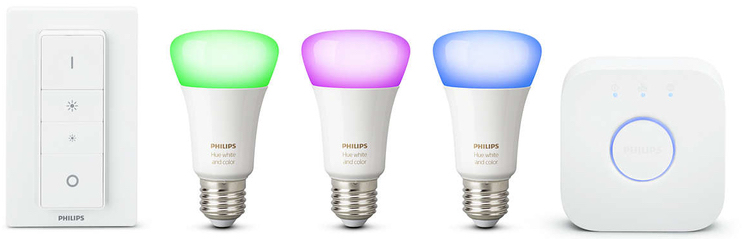
\includegraphics[width=0.9\textwidth]{images/Chapter_04/philips-hue.jpg}
	\caption{A Philips Hue dimmer switch, three color light bulbs and the Hue Smart Hub}
	\label{fig:philips-hue}
\end{figure}

\subsection{LG SmartThinQ}
LG SmartThinQ groups the range of Wi-Fi enabled home appliances made by the company LG, including refrigerators, dishwashers,
vacuum cleaners or air purifiers, between others. As of September 2017, they were the most extensive range of devices of their kind.\cite{lgSmartThinq}

Unlike Philips Hue, SmartThinQ devices do not require a bridge to work. They can be controlled from the mobile phone and, in some
cases, like in the refrigerators, they include a touchscreen to interact with the device. However, LG does not provide any extra device
or virtual assistant to interact with them, though they are manageable through Amazon Alexa and Google Assistant. A standard setup
with this system will follow a hybrid architecture, as some devices are also their controllers, but there can also be external controllers.

\subsection{Samsung SmartThings}
Samsung SmartThings is a home automation system composed by a series of applications for the Samsung mobile phones, Samsung
TVs and Samung refrigerators. It is even possible to do small management tasks from Samsung smartwatches, called Galaxy Gear. It 
uses the cloud to synchronize all the applications, in order to have the most recent information in all of them. This makes it necessary 
for the user to have a Samsung account.\cite{samsungSmartthings}

Unlike the previous systems, SmartThings is not a specific system for a range of devices from the same maker, but it is more aimed
to provide an effective interconnection between devices from different makers, as long as they are compatible with their system.
The SmartThings Smart Home Hub is necessary in order to use Samsung SmartThings. It is a bridge that supports common home 
automation protocols, like Zigbee or Z-wave, essential to manage some devices that only use these protocols. It also provides 
comprehensive automation options.\cite{smartHomeBeginner} The usage of the Hub makes the architecture of this system centralized.

Furthermore, SmartThings is not yet compatible with many commercial devices, and the restrictions imposed by Samsung forces the
user to stick to their environment. In addition, the system is not open source, so making any modification apart from the ones that
Samsung allows is impossible. Also, users are forced to purchase the Smart Home Hub, which makes it necessary to have an additional
device, unlike other similar systems. The system is compatible with Bixby, the virtual assistant from Samsung.

\subsection{Google Home}
Introduced at Google I/O 2016, the annual Google developer conference, \textit{Google Home} is the name of Google's smart speaker, 
which is Google's biggest insight into home automation technology. Its aim is to work with all the possible smart home devices, so it 
follows the same idea as the Samsung SmartThings system, being a \textit{maker-independent} system, as long as, of course, devices 
are compatible with it. Also, Google Home brings all the functions of Google Assistant to the smart speaker.

The main difference with SmartThings is that this system is mainly voice-driven. The home automation layer is pushed down to just 
one more function of the virtual assistant, and Google does not even provide a graphical interface to manage the smart devices.
Anyway, normally the makers of each device provide a mobile application from where users can manage their devices in a more
user-friendly interface, but having a centralized view is a desirable feature. On the bright side, all Google devices that support
Google Assistant can automatically control smart home devices. 

The number of compatible devices with the Google Assistant, unlike SmartThings, is very high, and almost any new smart home 
device is tagged as compatible with it.

\subsection{Apple HomeKit}
HomeKit is the result of Apple's efforts to create a home automation environment adapted to its devices. It has been also made to work
with a wide range of devices, but in this case, Apple included some notable security policies, with the goal of achieving the highest 
security and privacy. In fact, all HomeKit devices need to be approved by Apple first.

On iPhone and Mac computers (starting with macOS Mojave), Apple includes an application called Home, which displays all 
of the smart home devices in a convenient way and lets people organize and manage them. In addition, it is also possible to establish 
automation rules, based on the user's location, time of day, actions or even occupancy of the house. Furthermore, Apple also provides
integration with their personal assistant, Siri. As it happens with the Google Assistant, all Apple devices configured with the same Apple 
ID will have the same information automatically synchronized.\cite{appleIOSHome} Usually, systems made under Apple HomeKit will follow
a decentralized architecture.

Although this is a very comprehensive home automation system, the number of compatible devices is not as high as in other options. 
Apple has been lately working on promoting their home automation system and their assistant by introducing the HomePod, their smart
speaker with Siri.

\subsection{Somfy}
Somfy is a French company founded in 1960, which since the 1980s has been devoted to the construction of home automation systems.
They have implemented their solutions in important places, like the United Nations Headquarters or the Vancouver Convention Center 
and have created their own home automation technologies, such as \textit{Radio Technology Somfy (RTS)} and \textit{Somfy Digital 
Network (SDN)}.\cite{somfyOurStory}

Their range of products goes from control devices (as hand-held remotes, mobile applications and wireless switches) and sensors (sunlight,
temperature, wind) to blinds, lightning systems and other smart home utilities. Unfortunately, the control devices only work with Somfy 
devices. The system follows a hybrid architecture, where each device is a controller, but there can also be extra controllers, like the 
hand-held remotes.
\\~\\

In addition to the previous domotic systems, which are proprietary, there are also open source and more customizable solutions that, 
although they may require more time in their configuration, are much more adaptable to the needs of the user. I will explore three of
the most popular: openHAB, Home-Assistant.io and Jeedom.

\subsection{OpenHAB}
OpenHAB, the acronym for Open Home Automation Bus is an open source, technology agnostic home automation platform which runs
as the center of the smart home. \cite{openHABDocs} This means that its aim is to integrate different home automation systems into
a single one. It allows the user to configure almost every aspect of the system, providing a common interface and a uniform approach 
to automation rules.

In its most recent version, openHAB 2, it has implemented new user interfaces that automate many processes, so it is almost unnecessary
to write a single line of code, making the system more attractive to all types of users. OpenHAB needs to be installed in a computer that 
will act as a server in the local network, making the system accessible via HTTP. It also offers more connectivity options that I will explore 
in the following chapters.

OpenHAB's compatibility is somewhat limited when it comes to home automation devices, but it supports Apple HomeKit and common 
protocols, such as ZigBee and Z-Wave, to get rid of specific gateways from other systems.\cite{openHABAddons} 

\subsection{Home-Assistant.io}
Home-Assistant.io, or simply Home Assistant, is a open source home automation platform running on Python 3. Based on a distribution
called \textit{Hass.io}, it creates a secured local server in the computer where it is installed. It is accessible via HTTP and also includes
a web user interface that will automate the process of discovering and configuring devices. In terms of functionality, it is very similar to 
openHAB, although it might be a little simpler for some users, as it uses the YAML syntax for configuration, while openHAB has its own.

Its functionality is organized in \textit{Components}, the name that Home Assistant gives to any add-on, which will add a compatibility
layer with a device, system or service. They are fully backed by the Home Assistant community and they are similar in number and type to
what openHAB provides, but with very interesting additions, including Wink and Arduino. 

\begin{figure}
	\centering
	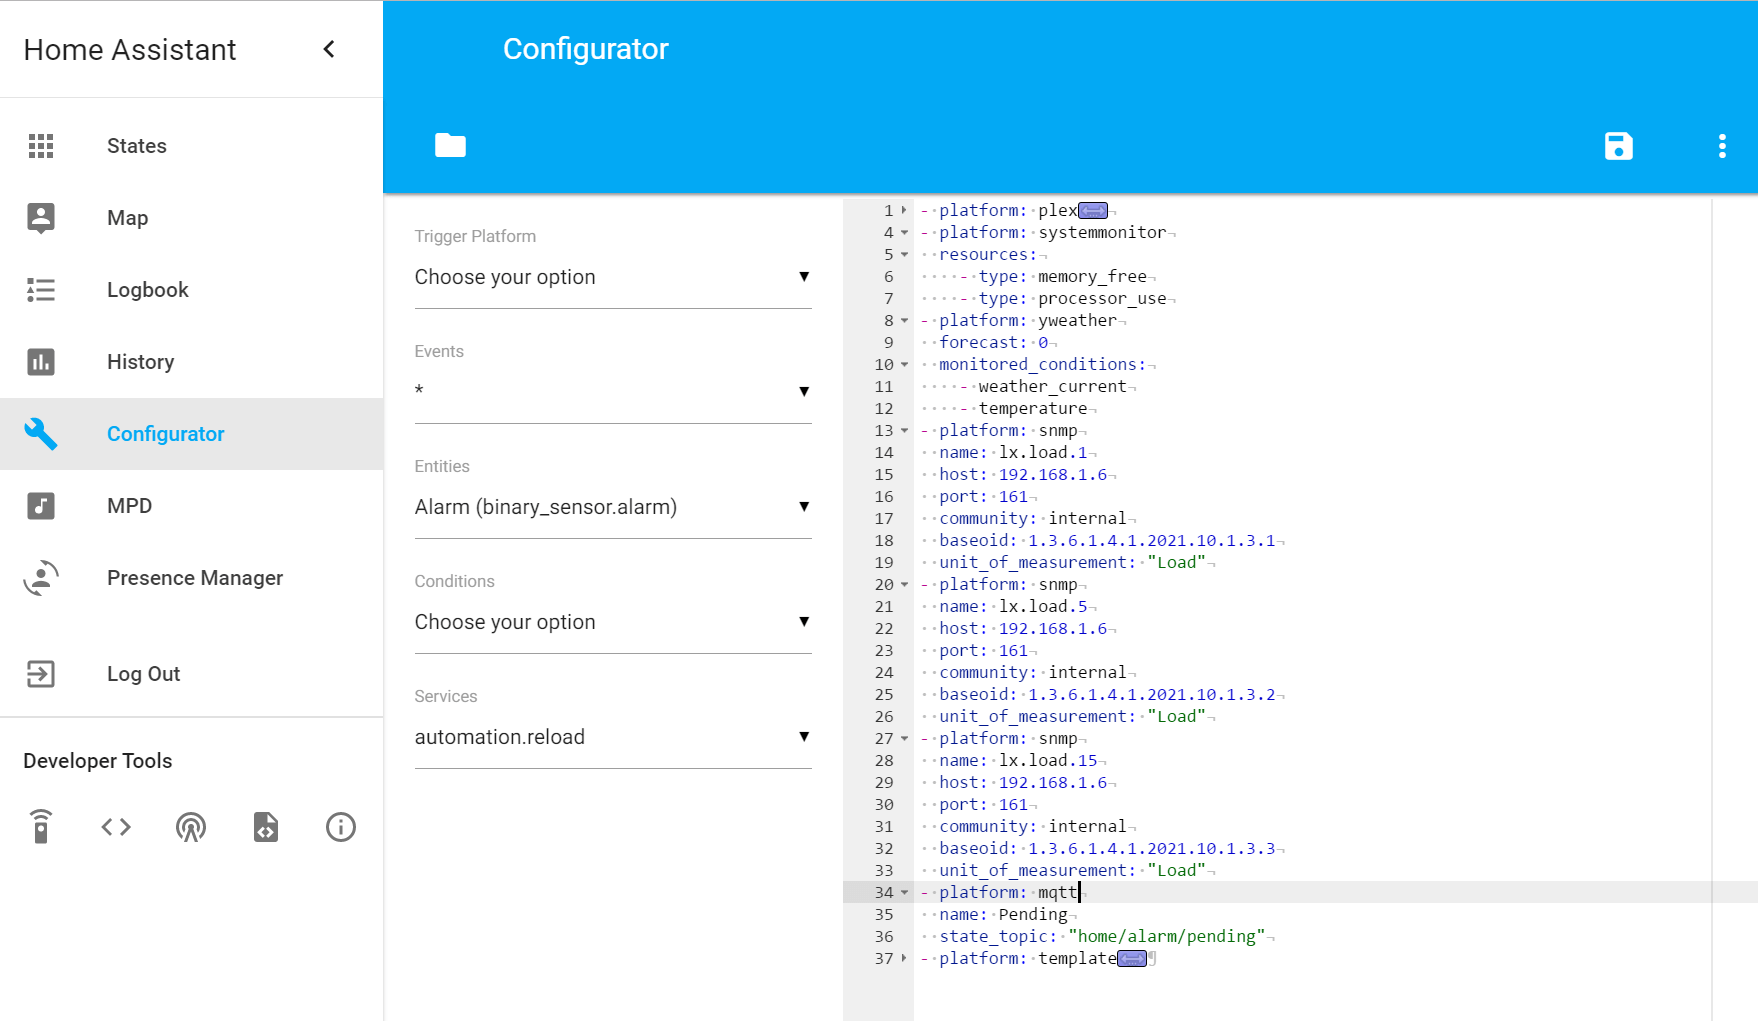
\includegraphics[width=0.9\textwidth]{images/Chapter_04/home-assistant-configuration.png}
	\caption{Home-Assistant.io web user interface}
	\label{fig:home-assistant-configuration}
\end{figure}

\subsection{Jeedom}
Jeedom is a open source, multi-protocol, autonomous and customizable home automation software. It is aimed for individuals and
professionals, and provides custom support for both. They also sell what they call \textit{Boxes}, which are small computers with
Jeedom pre-installed, although their software can be installed on any Linux system. Jeedom also provides mobile phone apps for Android
and iOS, which connect to the Jeedom system by scanning a QR code. As in the previous platforms, they also provide the \textit{Jeedom Market},
from where users can add new features to their system.

Also, there are different Jeedom versions, which are called \textit{Service packs}. There is the free and open source version, which
includes the lowest number of functionalities. Then, the other versions can be purchased, although some of them come with their Boxes,
and they include dynamic DNS and HTTPS, the mobile application for free or more plugins offered, among other things.

Although the free version is fully open source, the limitations that it has and the obligation to pay in order to have the \textit{full 
experience}, could annoy some users and make them lean towards other platforms.
\\~\\



\section{Voice Assistants}


% Incluir dispositivos que he estudiado, sistemas domóticos y alternativas a openHAB, asistentes de voz, etc
% Ejemplo de comparación entre asistentes de voz: https://en.wikipedia.org/wiki/Virtual_assistant